\chapter{Grundlagen}
\label{theory}

Dieses Kapitel soll einen Überblick über die zu simulierenden Prozesse und benutzten Simulationsmethoden geben.
Dazu stellt Abschnitt~\ref{depositions} das Prinzip von Gasphasenabscheidungen vor, Abschnitte~\ref{md} und~\ref{kmc} behandeln jeweils die Simulationsmethoden der Molekulardynamik und Kinetischen Monte-Carlo-Simulationen.
Zuletzt geht Abschnitt~\ref{datastructures} auf die verschiedenen Datenstrukturen ein, die genutzt werden, um effiziente Simulationen großer Simulationsräume zu ermöglichen.

\section{Gasphasenabscheidungen}

Gasphasenabscheidungen sind eine Klasse von Verfahren, bei denen dünne Schichten durch physikalische oder chemische Prozesse aus der Gasphase auf eine Oberfläche aufgetragen werden.
Sie teilen sich in \textbf{Physikalische Gasphasenabscheidung} (PVD, Physical Vapor Deposition), \textbf{Chemische Gasphasenabscheidung} (CVD, Chemical Vapor Deposition) und \textbf{Atomlagenabscheidung} (ALD, Atomic Layer Deposition) auf, die im folgenden betrachtet werden.

Ihnen ist allgemein, dass einzelne Atome oder Moleküle auf der Oberfläche aufkommen, dort physikalisch oder chemisch adsorbiert werden und eventuelle Nebenprodukte aus dem Reaktor gespült werden, wodurch mit vorhersehbarer Rate eine dünne Schicht des Zielmateriales aufwächst.
Tabellen \ref{tab:deposition-comparison} und \ref{tab:deposition-materials} stellen jeweils Charakteristiken und mögliche Materialien für die drei Prozesse dar.

\begin{figure}
  \centering
  \def\svgwidth{\textwidth}
  \input{img/reactors.pdf_tex}
  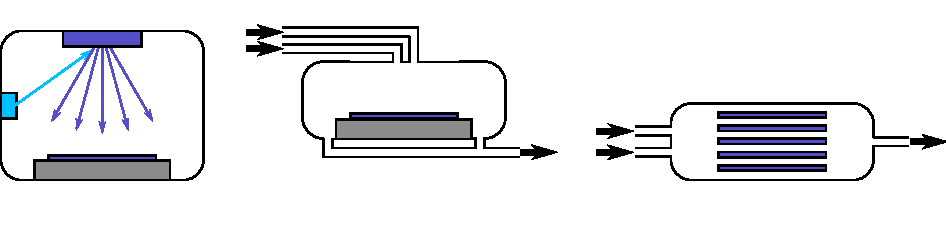
\includegraphics[]{reactors}
  \caption[Abscheidungskammern und -reaktoren]{Abscheidungskammern und -reaktoren}
  \label{fig:reactors}
\end{figure}

\begin{table}
  \centering
  \begin{tabularx}{\textwidth}{|X|ccc|}
    \hline
    Prozesscharakteristiken & \textbf{PVD} & \textbf{CVD} & \textbf{ALD} \\
    \hline
    reaktiv &  & \cmark & \cmark \\
    kontinuierlich & \cmark & \cmark & zyklisch \\
    Gas-Edukte & Atome, Moleküle & Precursor-Moleküle & Precursor-Moleküle \\
    \# Edukte & 1 & 1+ & 2+ \\
    Nebenprodukte & & \cmark & \cmark \\
    Wachstumsrate & $\sim t$ & $\sim t$ & $\sim n_\text{cyc.}$ \\
    \hline
  \end{tabularx}
  \caption[Prozesscharakteristiken der Abscheidungsarten]{Vergleich der Abscheidungsarten}
  \label{tab:deposition-comparison}
\end{table}

\begin{table}
  \centering
  \begin{tabularx}{\textwidth}{XXXXXXXXX}
    & \angled{Metalle} & \angled{Legierungen} & \angled{Metalloxide} & \angled{Nitride} & \angled{Chloride} & \angled{Silizium}  & \angled{Siliziumoxid} & \angled{Diamant} \\
    \hline
    \textbf{PVD} &\cmark&\cmark&&&&\cmark&&?\\
    \textbf{CVD} &\cmark&?&\cmark&\cmark&\cmark&\cmark&?&?\\
    \textbf{ALD} &\cmark&?&\cmark&\cmark&\cmark&\cmark&\cmark&\cmark\\
  \end{tabularx}
  \caption[Mögliche Produkte der Abscheidungsarten]{Mögliche Produkte der Abscheidungsarten. Weitergehende Informationen finden sich in der Literatur für PVD\cite{asd}, CVD\cite{asd} und ALD\cite{puurunen_surface_2005}.}
  \todo[inline]{Referenzen für abgeschiedene Systeme}
  \label{tab:deposition-materials}
\end{table}

\subsection{Physikalische Gasphasenabscheidung}

PVD ist kontinuierlich und nicht reaktiv, arbeitet also mit Atomen oder Molekülen, die physikalisch auf der Oberfläche adsorbieren.
Beispielsweise werden beim Sputtering durch energiereiche Partikel (Argon-Plasma) einzelne Atome aus dem sogenannten Target geschlagen, die dann auf dem Substrat eine homogene, dünne Schicht bilden.
Durch die Nutzung mehrerer Targets (Cosputtering) oder mehrerer Atomsorten in einem Target lassen sich auch Legierungen und andere mehrelementige Materialien abscheiden.
\todo{Referenzen für alles}

\subsection{Chemische Gasphasenabscheidung}

CVD wächst durch chemische Adsorption eines oder mehrerer Precursor-Moleküles eine dünne Schicht auf dem Substrat auf.
Dazu werden die Precursorgase zeitgleich in den Reaktor geleitet, wo sie über die Substratoberfläche strömen und Reaktionen ermöglichen.
Die dabei entstehenden Nebenprodukte werden mit dem Gasstrom aus dem Reaktor geführt, um die aufwachsende Schicht nicht zu verunreinigen.
\todo{zu abrupter Übergang}

Passende Precursor-Kombinationen zu finden, gestaltet sich oft schwierig, da sie idealerweise erst auf der Oberfläche und nicht in der Gasphase reagieren und dabei inerte Nebenprodukte erzeugen sollen.
Weitere Kriterien wie Prozesstemperaturen, Energiebarrieren und komplizierte Reaktionspfade erschweren die Suche zusätzlich.
Im Gegensatz zu PVD kann CVD dafür auf allen Substraten, über deren Oberfläche ein kontinuierlicher Gasfluss möglich ist, eine dünne Schicht abscheiden.
Dies beinhaltet Stufen, Rillen und anderweitig strukturierte Substrate ebenso wie Poren durch das Substrat.

\missingfigure{Beispiel Precursor-Moleküle}

\subsection{Atomlagenabscheidung}

\begin{figure}
  \centering
  \def\svgwidth{\textwidth}
  \input{img/ald-schema.pdf_tex}
  \caption[ALD-Schema]{ALD-Schema: dsa ald}
  \label{fig:ald-schema}
\end{figure}

Als Variation von CVD entstand ALD \todo{Referenz} mit dem Ziel, dünne Schichten kontrolliert in einzelnen Atomlagen abzuscheiden.
Dazu werden zwei Precursorgase in wechselweisen Schritten in den Reaktor geleitet, zwischen denen Spülschritte mit inertem Gas verbleibende Moleküle und Nebenprodukte aus dem Reaktor spülen (Abbildung \ref{fig:ald-schema}).
So werden einerseits Gasphasenreaktionen vermieden, andererseits sorgt die Sättigung \todo{Grafik zur Sättigung} der Oberfläche mit Precursorliganden in jedem Precursorschritt für zyklen-begrenztes Schichtwachstum.
Anders als der Name vermuten lässt, werden aber normalerweise keine kompletten Monolagen in einem Zyklus aufgebracht.
Üblicherweise erreichen ALD-Prozesse bis zu 35\% \todo{referenz} einer Monolage, bedingt durch sterische Hinderung (Abbildung \ref{fig:steric}).
Die Wachstumsrate wird somit von dem Growth-per-Cycle-Wert (GPC) abgelöst, der angibt, wie stark eine Schicht im Schnitt pro Zyklus wächst.

Große Gruppen von Precursorliganden verhindern durch sterische Hinderung einen hohen GPC-Wert, weshalb kompakte Precursor bevorzugt untersucht werden. \todo{Referenz?}
Die Suche nach möglichen Precursorpaaren und Prozessparametern unterliegt ansonsten gleichen Anforderungen wie bei CVD.

Eine ausführlichere Übersicht zu Atomlagenabscheidung und mögliche Precursorpaare findet sich in Referenz \cite{puurunen_surface_2005}.

\begin{figure}
  \centering
  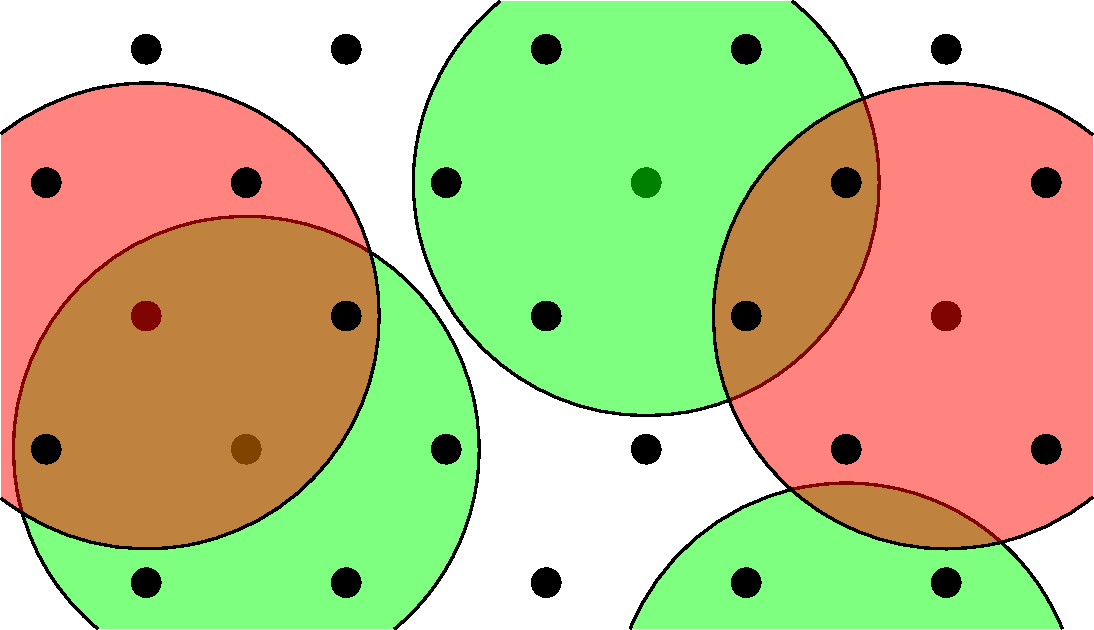
\includegraphics[width=0.5\textwidth]{sterichindrance}
  \caption[Sterische Hinderung]{Sterische Hinderung auf einem Gitter:
    Angelagerte Precursor-Liganden verhindern Reaktionen auf benachbarten Gitterpunkten.
    Überlagerungsfreie Positionen in größerem Abstand akzeptieren weiterhin Precursor-Reaktionen.
  }
  \label{fig:steric}
\end{figure}

\subsection{Simulation von Gasphasenabscheidungen}

\begin{table}
  \centering
  \begin{tabularx}{\textwidth}{XXXX}
    \hline
    Methode & Anwendungsfeld & Größenordnung & Grundlagen \\
    \hline
    Finite Elemente Methode (FEM) & Gasfluss und Verbrauch in Reaktoren & makroskopisch & Navier-Stokes-Gl., Reaktionskinetik \\
    Kinetic Monte Carlo (KMC) & Wachstums\-simulationen & mikroskopisch & Reaktionsraten, Gitternäherungen \\
    Molekular\-dynamik (MD) & Material\-unter\-suchungen & < 1.000.000 Atome & klassische Interaktionspotentiale \\
    Dichte\-funktional\-theorie (DFT) & Reaktionspfade & < 1.000 Atome & Elektronendichten \\
    \hline
  \end{tabularx}
  \caption[Ausgewählte Methoden zur Simulation von Gasphasenabscheidungen]{Ausgewählte Methoden zur Simulation von Gasphasenabscheidungen}
  \label{tab:deposition-simulations}
  \todo[inline]{Referenzen!}
\end{table}

Tabelle \ref{tab:deposition-simulations} stellt ausgewählte Simulationsmethoden für Gasphasenabscheidungen vor, die in der Praxis Anwendung finden.
Besonders auf atomarer Ebene sind viele Prozesse nicht vollends verstanden.
So ist der genaue Reaktionspfad für Precursorpaare oft nicht bekannt, obwohl sie seit Jahrzehnten erfolgreich eingesetzt werden.
Durch Simulationen will man diese Prozesse verstehen helfen und somit genauere Kontrolle über die abgeschiedenen Schichten erlangen.

Dichtefunktionaltheorie und Molekulardynamik stechen hier aufgrund ihrer atomaren Arbeitsweise besonders hervor.
DFT-Untersuchungen beschränken sich hier auf die Reaktionspfade von Molekülen, wo hingegen Molekulardynamik das fertige Material zu simulieren versucht.
In den letzten Jahren sind hingegen auch reaktive Formulierungen für Molekulardynamik aufgekommen\todo{Referenz}, die einen zentralen Bestandteil dieser Arbeit bilden.

\clearpage
\section{Molekulardynamik}

Molekulardynamik (MD) ist im Gegensatz zu quantenmechanischen Methoden eine klassische atomistische Methode, die zwar ungenauere Ergebnisse liefert, jedoch größere Systeme von bis zu einer Million Atome in akzeptabler Zeit rechnen kann.
Damit wird sie seit vielen Jahren erfolgreich in Physik, Chemie sowie in Materialwissenschaften genutzt, um System-, Molekül- und Materialeigenschaften zu bestimmen und Rückschlüsse auf reale Prozesse zu führen.
Somit existiert es eine Vielzahl gut erforschter Systeme, auf die im Rahmen dieser Arbeit aufgebaut wird.

\subsection{Formulierung}

\subsubsection{Allgemeines}

Als klassische Methode arbeitet Molekulardynamik mit Kraftfeldern, Massen.
So besteht ein System aus einer Vielzahl an Teilchen, die als Punktmasse angenähert werden, sowie einer universellen Zeit $t$.
Jedes Teilchen vereint also die Eigenschaften seiner Masse $m$, seines Impulses $\vec p$ und seiner Position $\vec r$.
Zusätzlich wirkt auf jedes Teilchen ein Kraftfeld $F(R)$ mit $R$ als aktuellem Systemzustand.

\subsubsection{Mikrokanonisches Ensemble (NVE)}

Es gilt für jedes Teilchen:

\begin{equation}
  \dot{\vec r} = {\vec p \over m}
\end{equation}

\begin{equation}
  \dot{\vec p} = m \vec a = F(R)
\end{equation}

\todo{Globale Formulierung!}

Zentral ist also das Kraftfeld $F(R)$, welches auf unterschiedliche Arten 

\subsubsection{Kanonisches Ensemble (NVT)}

Gegenüber dem mikrokanonischen Ensemble kommt im Kanonischen Ensemble noch ein Thermostat hinzu.
Dieses gleicht die mittlere Temperatur des Systemes an einen vorgegebenen Wert an.
Dies kann über harte Reskalierung der Atomgeschwindigkeiten (Berendsen-Thermostat), durch zufällige Stöße mit virtuellen Teilchen (Anderson-Thermostat) geschehen, oder durch einen zusätzlichen Reibungsterm, der auch negative Reibungskoeffizienten zulässt (Nosé-\-Hoover-\-Thermostat).

Unter Benutzung des \textbf{Berendsen-Thermostates} werden jeden Zeitschritt die Geschwindigkeiten aller Teilchen so skaliert, dass die Temperatur, die sich aus der kinetischen Energie über die Maxwell-Boltzmann-Verteilung für Gase ergibt, auf dem Zielwert gehalten wird:

\begin{equation}
  \overline{E_{kin}} = {1\over2} m\overline{v^2} = {d\over2}k_BT
\end{equation}

%% \begin{equation}
%% T = {m \overline{v^2} \over k_B d}
%% \end{equation}

Da dabei eine feste Temperatur erzwungen wird, ergibt dieses Thermostat kein kanonisches Ensemble, ist jedoch für große Systeme eine gute Näherung, die effizient berechnet werden kann.

Das \textbf{Anderson-Thermostat} hingegen arbeitet näher an der Idee des kanonischen Ensembles, über die Systemgrenzen hinweg Energie und somit Temperatur durch Teilchenstöße auszutauschen.
Dabei wird für die Zahl der Stöße pro Zeitschritt eine Poissonverteilung angenommen, Masse und Geschwindigkeiten der virtuellen Atome entsprechen der Zieltemperatur.
Zwar hat diese Vorgehensweise den Vorteil, mit einer geringen Anzahl an äußeren Einflüssen die Temperatur konstant zu halten, jedoch eignet es sich nur für die Betrachtung zeitgemittelter Größen.
Durch die Manipulation einzelner, zufälliger Atome können Trajektorien, insbesondere Abscheidungsorte und -konfigurationen stark beeinflusst werden.

Als Alternative eignet sich das \textbf{Nosé-Hoover-Thermostat}.
Dieses fügt dem Gesamtsystem einen zusätzlichen Freiheitsgrad $s$ hinzu, der die Temperatur beeinflusst.
Auf jedes Atom $i$ wirkt somit eine zusätzliche Reibungskraft entlang des Impulses:

\begin{equation}
  \dot{\vec p_i} = \vec{F_i} - s \vec{p_i}
\end{equation}

Der Reibungskoeffizient $s$ ändert sich dabei in Abhängigkeit vom System und kann dabei auch negative Werte annehmen:

\begin{equation}
  \dot s = {\tau \over M} \sum_i{{p_i^2 \over 2m_i} - {Nd \over k_BT}}
\end{equation}

\todo{tau hin oder weg?}

Damit fluktuiert die Temperatur um den Zielwert, wird also nicht fest erzwungen und folgt somit dem kanonischen Ensemble, wobei $\tau$ die Zeitskala angibt, auf der das System ins thermische Gleichgewicht übergeht.
In vielen Softwarepaketen für Molekulardynamiksimulationen dient das Nosé-Hoover-Thermostat als Standardthermostat.

\subsubsection{Großkanonisches Ensemble (NPT)}

Zusätzlich zu einem Thermostat kommt im großkanonischen Ensemble ein Barostat zum Einsatz.
Dieses reguliert über Reskalierung des Simulationsraumes unter periodischen Randbedingungen den mittleren Druck des Systemes.
Dadurch lassen sich periodische Strukturen wie Kristalle frei relaxieren, ohne ihnen eine feste Dichte aufzuzwingen.
Andererseits lassen sich auch Systeme unter großen Drücken untersuchen.

Die Methoden des Barostats gleichen dem des Thermostats, wobei hier nicht die einzelnen Atome, sondern deren relativer Abstand von einander durch Skalierung der Raumposition manipuliert wird.
Als Voreinstellung kommt üblicherweise wieder ein Nosé-Hoover-Barostat zum Einsatz, wobei aufgrund seiner Einfachheit auch Berendsen-Barostate genutzt werden.
Der Druck wird dabei über die Virialgleichung \todo{für ideale Gase?} ermittelt:

\begin{equation}
  PV = Nk_BT + \frac{1}{d} \sum_{i=1}^N{\vec{r}_i \cdot \vec{F}_i}
\end{equation}

\subsubsection{Minimierung durch Konjugierte Gradienten (CG-Minimierung)}

\begin{figure}[!b]
  \centering
  \def\svgwidth{0.8\textwidth}
  \input{img/cg-gradient.pdf_tex}
  \caption[CG-Methode]{Klassische Minimierung durch konjugierte Gradienten:\\
a) Optimale Schrittlänge\\
b) Kleine Schrittlänge $\Rightarrow$ viele unnötige Schritte\\
c) Große Schrittlänge $\Rightarrow$ langsames Konvergenzverhalten
}
  \label{fig:cg-gradient}
\end{figure}

Zur Energieminimierung, welche der Strukturoptimierung dient, wird häufig die \textbf{Methode der konjugierten Gradienten} angewandt.
Man sucht dabei in der Grundvariante ausgehend von einem beliebigen Startpunkt $\vec x_0$ das Minimum der im Suchbereich stetigen Funktion $f(\vec x)$ durch schrittweise Annäherung entlang des Gradienten:

\begin{gather}
  \vec s_i = \Delta\vec x_i = \nabla f(\vec x_{i-1})\\
  \vec x_i = \vec x_{i-1} - \alpha \vec s_i
\end{gather}

Der zusätzliche Parameter $\alpha$ legt dabei die Schrittweite fest.
Mögliche Abbruchkriterien können dabei die Differenz zwischen zwei Schritten ($\left|\vec x_i - \vec x_{i-1}\right| < x_\text{tol}$), die maximale Änderung eines Vektorelementes ($\max_k{\left|x_{i,k} - x_{i-1,k}\right|} < x_\text{tol}$), die Stärke des Gradienten ($\left|\nabla f(\vec x_{i-1})\right| < x_\text{tol}$), eine Anzahl an Zeitschritten ($i > i_\text{tol}$) oder eine Kombination daraus sein.

Dieser grundlegende Algorithmus stößt schnell anseine Grenzen, wenn man allgemeine, nichtlineare Funktionen minimieren möchte.
Dafür führt man mehrere Änderungen ein:
Einerseits ersetzt man den Sprung durch eine Minimierung entlang der Schrittrichtung (Gleichungen \ref{eq:cg-linesearch1} und \ref{eq:cg-linesearch2}).
Andererseits ändert man die Schrittrichtung in Abhängigkeit vorheriger Schritte leicht ab (Gleichungen \ref{eq:pr1} und \ref{eq:pr2}).
Hier wird die Polak-Ribière-Variante vorgestellt1, die standardmäßig in LAMMPS zum Einsatz kommt, jedoch existieren weitere gleichwertige Methoden.

\begin{gather}
  \label{eq:cg-linesearch1}
  \min_\alpha f(x_i+\alpha \vec s_i) \rightarrow \alpha_i \\
  \label{eq:cg-linesearch2}
  \vec x_i = \vec x_{i-1} - \alpha_i \vec s_i\\
  \label{eq:pr1}
  \vec s_i = \Delta \vec x_i + \beta_i \vec s_{i-1}\\
\end{gather}
\begin{equation}
  \label{eq:pr2}
  \beta_i = \max \left(0, \frac{\Delta \vec x_i \cdot \left(\Delta \vec x_i - \Delta \vec x_{i-1}\right)}{\Delta \vec x_{i-1} \cdot \Delta \vec x_{i-1}}\right) \text{ (Polak-Ribière)}
\end{equation}

Diese Anpassungen verbessern einerseits das erwartete Konvergenzverhalten, andererseits stabilisieren sie den Optimierungsalgorithmus gegenüber Nichtlinearitäten und Unstetigkeiten\todo{Referenz? Lüge?}.

\subsubsection{Weitere Minimierungsmethoden}

Es stehen noch weitere Minimierungsalgorithmen zur Verfügung, wie beispielsweise die Klasse der Newton-Verfahren.
Obwohl diese auf dem Papier schneller konvergieren, sind für jeden Iterationsschritt durch die Berechnung der Hesse-Matrix mehr Rechenoperationen notwendig, so dass reale Berechnungszeit und Speicherverbrauch gegenüber CG-Methoden oft im Nachteil sind.
\todo{Referenz für Interessierte}

\subsection{Kraftfelder}

Basis aller im vorherigen Abschnitt vorgestellten Methoden sind stets Kraftfelder, die die gewünschte Struktur darstellen können.
Hierfür gibt es eine Vielzahl an verschiedenen Formulierungen, für die es jeweils verschiedene Parametrisierungen gibt, um bestimmte Systeme und Umgebungen zu betrachten.

\subsubsection{Paar-Potentiale}

\missingfigure{Lennard-Jones, Buckingham, Hartkugel}

Das klassische MD-Potential ist das Paarpotential, welches eine Interaktion zwischen zwei benachbarten Atomen modelliert.
Stellvertretend sind beispielsweise das Lennard-Jones-Potential zur Darstellung von allgemeinen Fluiden (Gleichung \ref{eq:lennardjones}) oder das damit verwandte Bucking\-ham-Potential.

\begin{equation}
  \label{eq:lennardjones}
  V_{LJ}(r_{ij}) = 4 \epsilon \left[\left(\frac{\sigma}{r_{ij}}\right)^{12} - \left(\frac{\sigma}{r_{ij}}\right)^{6}\right]
\end{equation}
\begin{equation}
  \label{eq:pairforce}
  \vec F_{ij}(\vec r_{ij}) = \vec\nabla V(r_{ij})
\end{equation}
\begin{equation}
  \label{eq:pairenergy}
  E = \sum_i\sum_{j \neq i}{V_{LJ}\left(r_{ij}\right)}
\end{equation}

Andere Potentiale enthalten weitere Parameter oder tabellierte Werte, mit denen spezielle Probleme genauer betrachtet werden können.
Das allgemeine Problem der Klasse der Paarpotentiale ist ihre Schlichtheit.
So lassen sie sich schwer an realistische Strukturen fitten und können oftmals nur ein Material in einem Szenario darstellen, wobei sie allerdings schnell sind.

\subsubsection{N-Teilchen-Potentiale}

N-Teilchen-Potentiale  erweitern Paarpotentiale um weitere Terme, die von einer festen Anzahl an Teilchen abhängen, beispielsweise Winkel- und Torsionsabhängigkeiten.

\begin{equation}
  \label{eq:nbody-energy}
  E = \sum_i\sum_{j \neq i}{V_2\left(r_{ij}\right)} + \sum_i\sum_{j \neq i}\sum_{i \neq k \neq j}{V_3\left(r_{ij}, r_{ik}, \theta_{ijk}\right)}
\end{equation}
\todo{letzte Summe: Indizes aufspalten}

Obwohl sich mit N-Teilchen-Potentialen komplexere Systeme betrachten lassen, zeigen sie die gleichen Schwachstellen wie Paarpotentiale.
Zwar gibt es erfolgreiche \todo{kommerzielle} Anpassungen für Biomoleküle (\todo{CHARMM} \todo{GROMACS} \todo{AMBER}), die allerdings nicht auf andere Stoffsysteme übertragbar sind.

\subsubsection{Embedded Atom Model}

Das Embedded Atom Model (EAM) für jedes Atom $i$ besteht aus einem Paarpotential $V_{\alpha\beta}(r_{ij})$ sowie einer Einbettungsfunktion $F_\alpha$, die die Energie jedes Atomes in Abhängigkeit der angenäherten Elektronendichte $\rho_\beta(r_{ij})$ in der Umgebung modelliert (Gleichung \ref{eq:eam-energy}).\todo{Referenz}
So lassen sich insbesondere metallische Materialien und Oberflächen simulieren.
$\alpha$ und $\beta$ stellen dabei verschiedene Atomsorten dar, allerdings lassen sich auch mit dieser umfangreicheren Formulierung hauptsächlich reine Metalle simulieren.
Für diese findet man allerdings passende Parametrisierungen\todo{Referenz auf Datenbank und passende Paper}, die im Gegensatz zu den meisten Potentialen sowohl thermisches Verhalten als auch Strukturen recht gut modellieren \todo{Referenz auf separates Ergebniskapitel}.

\begin{equation}
  \label{eq:eam-energy}
  E = \sum_i\left[F_\alpha\left(\sum_{j\neq i}{\rho_\beta\left(r_{ij}\right)}\right) + \frac{1}{2}\sum_{j\neq i}{V_{\alpha\beta}\left(r_{ij}\right)}\right]
\end{equation}

\subsubsection{Modified Embedded Atom Model}

Um die Einschränkung des reinen EAM-Potentials zu umgehen, wurde das Modified Embedded Atom Model (MEAM) erforscht (Gleichung \ref{eq:meam-energy}). \todo{Referenz auf Baskes}
Mit diesem lassen sich auch Metalloxide, Legierungen und andere Mischsysteme untersuchen\todo{Referenz}.

\todo{Wie funktioniert es?}

\begin{equation}
  \label{eq:meam-energy}
  E = \sum_i\left[F_\alpha\left(\bar{\rho_i}\right) + \frac{1}{2}\sum_{j\neq i}{V_{ij}\left(r_{ij}\right)}\right]
\end{equation}

Wie beim EAM-Potential sind die eigentlichen Berechnungen in den einzelnen Funktionen versteckt, die auf umfassende Weise die Elektronendichten zu modellieren versuchen.
Dafür ist vorher eine umfangreichere Parametrisierung notwendig, die an eine Vielzahl von Strukturen gefittet werden muss.

\subsubsection{Reactive Force Fields}

\todo{Referenz}
Reactive Force Fields (ReaxFF) wurden mit der Idee erdacht, bisher unmögliche Simulationen in Molekulardynamik mit größeren Systemen darstellen zu können.
Dafür fließt eine Vielzahl an Einflüssen in die Potentialgestaltung ein, beispielsweise Van-der-Waals-Kräfte und elektrostatische Kräfte, allerdings ist der zentrale Gedanke die Modellierung von Über- und Unterkoordination eines Atomes in seiner Nachbarschaft unter Ladungsaustausch.
Somit lassen sich Bindungen während der Simulation dynamisch formen und lösen und dadurch ganze Reaktionen zwischen verschiedenen Molekülen simulieren.

\begin{align}
  \label{eq:reax-formulation}
  E_\text{system} &= E_\text{bond} + E_\text{lp} + E_\text{over} + E_\text{under} + E_\text{val} + E_\text{pen} + E_\text{coa} + E_\text{C2} \\
\nonumber  & + E_\text{tors} + E_\text{conj} + E_\text{H-bond} + E_\text{vdWaals} + E_\text{Coulomb}
\end{align}

Die meisten Terme der Gesamtenergie werden über die Bindungsordnung berechnet, die über Beiträge für $\sigma$-, $\pi$- und Doppel-$\pi$-Bindungen aus dem Bindungsabstand errechnet wird.
Einige werden durch Taper-Korrektur\todo{ref} in der Nähe des Cutoff-Abstandes auf 0 gesenkt, um Diskontinuitäten zu vermeiden und einen fließenden Übergang zwischen Bindungszuständen zu ermöglichen.

\todo{Referenz auf Equations\_Reax.pdf}

\begin{table}
  \begin{tabularx}{\textwidth}{llX}
    \hline
    Term & Beitrag & Kommentar \\
    \hline
    $E_\text{bond}$ & Bindungsenergien & Berechnung über Bindungsordnung\\
    $E_\text{lp}$ & freie Elektronenpaare & über Bindungsordnungssumme am Atomzentrum\\
    $E_\text{over}$ & Überkoordinationen & unter Ausschluss freier Elektronenpaare\\
    $E_\text{under}$ & Unterkoordinationen & nur bei unterkoordinierten $\pi$-Bindungen\\
    $E_\text{val}$ & Bindungswinkel & Optimum abhängig von Elektronenkonfiguration\\
    $E_\text{pen}$ & Strafenergien & Fehlerkorrektur bei Winkeln mit Doppelbindung\\
    $E_\text{coa}$ & Drei-Teilchen-Konjugationen & Stabilisierung von NO$_2$-Gruppen\\
    $E_\text{C2}$ & Dreifachbindungskorrektur & Stabilisierung der Dreifachbindung von C$_2$\\
    $E_\text{tors}$ & Torsionsbarrieren & \\
    $E_\text{conj}$ & Vier-Teilchen-Konjugationen & Konjugation bei Kohlenwasserstoffen\\
    $E_\text{H-bond}$ & Wasserstoffbrücken & \\
    $E_\text{vdWaals}$ & Van-der-Waals-Kräfte & \\
    $E_\text{Coulomb}$ & Coulomb-Kräfte & \\
    \hline
  \end{tabularx}
  \caption[ReaxFF Energiebeiträge]{ReaxFF Energiebeiträge aus Gleichung \ref{eq:reax-formulation}}
  \label{tab:reax-energies}
\end{table}

Wie aus Gleichung \ref{eq:reax-formulation} und Tabelle \ref{tab:reax-energies} hervor geht, wurden das ReaxFF-Potential ursprünglich für Reaktionen von organischen Molekülen entwickelt, ist aber vielseitig genug, eine Vielzahl anderer Materialien simulieren zu können.
Die unterstützten Stoffgruppen hängen dabei stark von den Strukturen ab, an die die Parametrisierung gefittet wurde.
Auch, wenn alle notwendigen Atomsorten unterstützt werden, kommt es häufig vor, dass der zu untersuchende Stoff bei der Parametersuche nicht beachtet wurde und somit nicht darstellbar ist.

In den letzten fünf Jahren haben Reactive Force Fields jedoch langsam an Aufmerksamkeit gewonnen, so dass die Zahl spezialisierter Parametrisierungen wächst.
Es gibt auch Bestrebungen, sich ergänzende ReaxFF-Parametrisierungen zu kombinieren und somit mit einer Parametrisierung jedes gewünschte System betrachten zu können.
Besonders in kommerzieller MD-Software\todo{Referenz auf GULP} versucht man so, dem Nutzer unnötige Arbeit abzunehmen.
Es muss sich jedoch noch zeigen, ob dieser Ansatz zufrieden stellende Ergebnisse liefern kann.

\subsubsection{Allgemeine Probleme}

\textbf{Parametrisierung}:
Da Molekulardynamik keine ab-initio-Methode ist, sondern jedes Potential erst an experimentelle oder numerische Daten angepasst (gefittet)\todo{was nun?} werden muss, sollte die Herkunft jeder Parametrisierung bei seiner Nutzung bedacht werden.
\todo{kulkarni: Kritische Betrachtung seiner Trainingsstrukturen}
\\\\
\textbf{Übertragbarkeit}:
Je nach Potentialart lassen sich viele Parametrisierungen nicht vermischen oder auf andere Probleme übertragen.
\\\\
\textbf{Analysemethoden}:
Im Normalfall sind Potentiale entweder für strukturelle oder thermische Größen optimiert.
Mit einem rein strukturellen Potential lassen sich also keine thermischen Größen und Phasenübergänge verlässlich ermitteln.
\\\\
\textbf{Reaktionen}:
Mit der Ausnahme des ReaxFF-Potentiales lassen sich per Molekulardynamik keine Reaktionen betrachten.
\\\\
\textbf{Annäherungen}:
\todo{Was hast du hier gedacht, Erik?}

\subsection{Auswertung}

\subsubsection{Relaxierungen}

\subsubsection{Struktur}

Zur Auswertung einer Struktur bietet sich zuerst eine visuelle Beurteilung an, die mit entsprechenden Programmen vorgenommen werden kann.
Damit können grobe Defekte ausgeschlossen werden.

\subsubsection{Dichte}

Die Dichte lässt sich bei periodischen Strukturen nach über Volumen und 

\subsubsection{Radiale Verteilungsfunktionen}

\subsubsection{Oberfläche}

Die Oberfläche einer Struktur gibt Hinweise auf angelagerte Molekülgruppen, Rauheit, Porösität und Bildung reinatomiger Cluster.
Bei großen, glatten Strukturen reicht oft ein Schnitt entlang einer Hauptachse, um Bulk und Oberfläche zu trennen.
In den verbliebenen Fällen lässt sich zu diesem Zweck eine Alpha-Form per Delaunay-Triangulation bestimmen. \todo{Referenz auf Delaunay-Section}
Die eigentlichen Untersuchungen beschränken sich dann auf eine Zählung der Bindungen und Atomsorten, Radiale Verteilungsfunktionen, Oberflächenmessung oder Höhenabweichung vom Mittelwert.

\subsubsection{Reaktionen}



\subsection{Software}

Für molekulardynamische Simulationen gibt es sowohl kommerzielle als auch freie Softwarepakete, die einige Parametersätze mitbringen.
Tabelle \ref{tab:mdsoftware} stellt eine Auswahl daraus dar.

\begin{table}
  \begin{tabularx}{\textwidth}{llX}
    \hline
    Paket & Rechteinhaber & Kommentare \\
    \hline
    LAMMPS & SANDIA & quelloffen, CLI-bedienbar, Bibliothek, eigene Potentiale möglich \\
    Materials Studio GULP & Accelrys & Tief in graphischer Oberfläche verankert \\
    AMBER & University of California & verschiedene Biomoleküle \\
    CHARMM & Accelrys & Proteine \\
    GROMACS & Uppsala University & Biomoleküle, quelloffen \\
    \hline
  \end{tabularx}
  \todo[inline]{References!}
  \todo[inline]{bessere Beschreibung!}
  \caption[MD-Software]{MD-Software}
  \label{tab:mdsoftware}
\end{table}


\clearpage
\section{Kinetic Monte Carlo-Methoden}

Kinetic Monte Carlo-Methoden bezeichnen zufallsbestimmte numerische Prozesse, bei denen das System eine Reihe von diskreten Zuständen durchläuft, die auf Basis einer Übergangswahrscheinlichkeit aus dem vorhergehenden Zustand zufällig gewählt werden.
Ursprünglich für die Simulation von  Diffusionsprozessen entwickelt, finden sie inzwischen in vielen Gebieten der Natur- und Ingenieurswissenschaften Anwendung, insbesondere auch für Nichtgleichgewichtssysteme wie  Oberflächenreaktionen und Schichtabscheidungen.

Die mathematische Formulierung folgt Markov-Ketten, die eine Abfolge von Zuständen $X_t$ aus einem abzählbar großen Zustandsraum $S$ darstellen. ASD

$$
X_t = S \forall t \geq 0
$$
$$
X_{t+\Delta t} = E(X_t, t)
$$
$$
\Delta t = - \frac{\ln(u)}{r_i}
$$


\clearpage
\section{Datenstrukturen}
\label{datastructures}

Zur Beschleunigung von atomistischen Simulationen mit Parsivald finden effiziente Algorithmen zur Suche und Manipulation von Atomen auf Basis verschiedener Datenstrukturen Anwendung, welche im Folgenden zwecks der Beschreibung von Atompositionen in teilperiodischen Simulationsräumen für Off-Lattice-KMC-Simulationen untersucht werden sollen.
Gegenüber optimalen Algorithmen für allgemeine Probleme, wie sie in verfügbarer Software genutzt werden, ermöglicht die genaue Modell- und Systemkenntnis die Abwägung der Häufigkeit von Operationen gegen deren Laufzeiten,
wodurch die Wahl der optimalen Datenstruktur zur Maximierung von Größe, Genauigkeit und Geschwindigkeit von Off-Lattice-KMC-Simulationen von Gasphasenabscheidungen ermöglicht wird.

\subsection{Numerische Voraussetzungen an Gasphasenabscheidungen}

Für eine effiziente KMC-Simulation werden für zu untersuchende Gasphasenabscheidungen folgende Voraussetzungen getroffen:
Zuerst sollten die KMC-Ereignisse \textbf{lokal}, also auf eine geringe Reichweite begrenzt sein.
Das bedeutet auch, dass die Atome über \textbf{niedrige Diffusionskoeffizienten} verfügen, was sich aus der Notwendigkeit ergibt, im statischen Gleichgewicht befindliche Bereiche des Simulationsraumes von atomistischen Simulationen auszuschließen.
Weiterhin werden \textbf{scharfe Phasengrenzen} vorausgesetzt, also zweidimensionale Grenzflächen, die sich durch eine vergleichsweise geringe Menge von Atomen darstellen lassen.
Zuletzt finden die Simulationen aus praktischen Gründen in \textbf{teilperiodischen Räumen} statt, also Räumen, die in der xy-Ebene periodisch, aber in z-Richtung beliebig ausgedehnt sein können.

%% Daraus ergeben sich jeweils Vor- und Nachteile für verschiedene Datenstrukturen, so dass etwa für die Vereinigung zweier disjunkter Triangulation (Stitching) in periodischen Räumen zusätzlicher Aufwand gegenüber nichtperiodischen Räumen betrieben werden muss.
%% Die größten Vorteile ergeben sich aus der Lokalität von Ereignissen, da so für die meisten Datenstrukturen nur kleine Teilstrukturen überprüft und aktualisiert werden müssen.

\subsection{Vergleich der Laufzeiten mit verschiedenen Datenstrukturen}

Als Datenstrukturen stehen \textbf{Atomlisten}, \textbf{Nachbarschaftslisten} (NB-Listen), lineares \textbf{Binning}, Binning in \textbf{Octrees}, \textbf{k-d-Bäume} und \textbf{Delaunay-Triangulationen} zur Auswahl.
%, von denen eine Auswahl in Abbildung~\ref{fig:datastructures} dargestellt ist.
In Anhang~\ref{appendix_dataoverview} werden diese knapp vorgestellt, wobei auf die drei zuletzt genannten in den folgenden Abschnitten näher eingegangen wird.

Atomistische KMC-Simulationen beschränken sich auf die Manipulations-Operationen zur \textbf{Einfügung}, \textbf{Modifikation} und \textbf{Entfernung} von Atomen, \textbf{Konstruktion} der Datenstruktur sowie auf die Suchoperationen der \textbf{Nachbarschaftssuche}, \textbf{Bereichssuche} und \textbf{Oberflächensuche}, die jeweils in Anhang~\ref{dataops} kurz beschrieben werden.
Die Effizienz dieser Operationen geht dabei aus deren asymptotischer Laufzeit hervor, welche üblicherweise in asymptotischer Notation (\BigO{}) angegeben wird.

Bei KMC-Simulationen überwiegen die drei Suchoperationen, da sie für jedes Ereignis beim Aufbau der KMC-Ereignislisten durchgeführt werden müssen, wo hingegen die Manipulationen nur für das tatsächlich durchgeführte Ereignis ausgeführt werden müssen.
Somit liegt das Auswahlkriterium der Datenstruktur bei der Effizienz ihrer Suchoperationen, mit Ausnahme der Nachbarschaftslisten und k-d-Bäume, deren Manipulationsoperationen für große Simulationsräume \todo{phrasing}zu langsam sind.
Die Ergebnisse der Laufzeit-Analysen der sieben Operationen auf den vorgestellten Datenstrukturen werden in Tabelle~\ref{tab:dataruntimes} zusammen gefasst, wofür Tabelle~\ref{tab:datasymbols} die verwendeten Symbole erklärt.

\begin{table}[!ht]
  \centering

  \caption{Abschätzung der Komplexität für verschiedene Datenstrukturen und Operationen}
  \label{tab:dataruntimes}
  \begin{tabularx}{\textwidth}{|X|*8c|}
    \hline
    \textbf{Datenstr.} & Konstr.         & Einfüg.         & Modif.          & Entf.           & Ortss.                     & NB-Su.              & Oberfl.        & RAM                         \\
    \hline
    Atomlisten         & \cG{$n$}        & \cG{$1$}        & \cG{$1$}        & \cG{$1$}        & \cR{$n$}                   & \cR{$n$}            & \cR{$n$}       & \cG{$n$}                    \\
    NB-Listen          & \cY{$n\log{n}$} & \cR{$n$}        & \cR{$n$}        & \cR{$n$}        & \cR{$n$}                   & \cG{$1$}            & \cR{$n$}       & \cR{$\frac{r_c^3}{s^3}n^2$} \\
    Binning            & \cG{$n$}        & \cG{$1$}        & \cG{$1$}        & \cG{$1$}        & \cG{$r_s^3$}               & \cG{$r_s^3$}        & \cR{$c$}       & \cY{$n+c$}                  \\
    Octree             & \cY{$n\log{c}$} & \cY{$\log{c}$}  & \cY{$\log{c}$}  & \cG{$1$}        & \cY{$r_s^3\log{c}$}        & \cY{$r_s^3\log{c}$} & \cY{$\log{c}$} & \cY{$n+c^\frac{2}{3}$}      \\
    k-d-Baum           & \cY{$n\log{n}$} & \cY{$\log{n}$}  & \cY{$\log{n}$}  & \cY{$\log{n}$}  & \cY{$r_s^3\log{n}$}        & \cY{$r_s^3\log{n}$} & \cY{$\log{n}$} & \cG{$n$}                    \\
    Delaunay           & \cY{$n\log{n}$} & \cY{$k\log{k}$} & \cY{$k\log{k}$} & \cY{$k\log{k}$} & \cG{$r_s^3+n^\frac{1}{3}$} & \cG{$r_s^3$}        & \cG{$1$}       & \cY{$nk$}                   \\
    \hline
    %Atomfeld          & \cG{$n$}        & \cG{$1$}        & \cG{$1$}        & \cG{$1$}        & \cR{$n$}                   & \cR{$n$}            & \cR{$n$}       & \cG{$n$}                    \\
  \end{tabularx}
  \vspace{1em}
  \hspace{0.15\textwidth}
  \begin{tabularx}{0.6\textwidth}{|C|C|C|}
    \hline
    \cG{optimal} & \cY{vertretbar} & \cR{ineffizient} \\
    \hline
  \end{tabularx}

  \vspace{1em}

  \oddrowcolors
  \caption{Symbole für Laufzeit- und Speicherabschätzungen}
  \label{tab:datasymbols}
  \begin{tabularx}{\textwidth}{|cX|cX|}
    \hline
    \textbf{Symbol} & \textbf{Bedeutung}                 & \textbf{Symbol} & \textbf{Bedeutung} \\
    \hline
    \BigO{}         & Worst-Case-Komplexität             & $n$             & Zahl der Atome     \\
    $k$             & Zahl von Nächstnachbarn            & $b$             & Zahl der Bins      \\
    $k_r$           & Zahl von Nachbarn mit $d \leq r_c$ & $r_c$           & Cutoff-Radius      \\
    $r_s$           & Suchradius                         & $s$             & lineare Raumgröße  \\
    \hline
  \end{tabularx}

\end{table}

\clearpage
\subsection{Effiziente Datenstrukturen}

Beim Vergleich der Datenstrukturen in Tabelle~\ref{tab:dataruntimes} stellen sich Octrees, k-d-Bäume und Delaunay-Triangulationen als Favoriten für Off-Lattice KMC-Simulationen heraus, die in den folgenden Abschnitten kurz eingehender vorgestellt und diskutiert werden sollen.
Der Speicherverbrauch der untersuchten Datenstrukturen ist praktisch linear und bildet deshalb kein Auswahlkriterium.
Wie Untersuchungen an Simulationsräumen verschiedener Größe zeigen, wird erst für \num{1.9e9} Atome die Grenze des Hauptspeichers erreicht (Abschnitt~\ref{goldscalability}).

\subsubsection{Octrees}
\label{dataoctree}

Octrees sind eine Optimierung raumfüllender orthogonaler Partitionierungen, wie sie üblicherweise für Binning-Methoden genutzt werden, bei der statt linearer Adressierung auf einen mehrdimensionalen Binärbaum zurück gegriffen wird, woher auch der Name stammt (1D: Binary Tree, 2D: Quadtree, 3D: Octree, etc.).
Der Simulationsraum wird rekursiv in jeweils 8 disjunkte geometrisch ähnliche Unterzellen halber Breite aufgeteilt, wodurch die eigentlichen Bins in der festen Tiefe $\frac{\log{c}}{d\log{2}}$ liegen.

Damit steigt die Adressierungszeit für einzelne Zellen auf \BigO{\log{c}}, doch werden nur die Bins allokiert, die tatsächlich gefüllt sind (Abbildung~\ref{fig:octree}), wodurch leere Superzellen bei Suchoperationen automatisch übergangen werden.
Als Resultat sind für Oberflächensysteme der Speicherbedarf und die Laufzeit von Suchoperationen eines dreidimensionalen Simulationsraumes auf die eines zweidimensionalen Systemes reduziert.
Theoretisch sind mit Access Caching, Bitweiser Adressierung, Surface Flagging oder Height Mapping noch weitere Anpassungen möglich, allerdings verbessert sich dabei nur der Laufzeitfaktor, nicht die asymptotische Laufzeit, weshalb sie nur am Rand genannt sein sollen.

%% \begin{algorithm}
%%   \begin{algorithmic}
%% %    \Input $atoms$ - Liste der Atome
%% %    \Input $size[3]$ - Größe des Simulationsraumes
%% %    \Input $depth$ - Tiefe des Octrees (Legt die Zellgröße fest)
%% %    \Assumption Alle Atome befinden sich im Simulationsraum
%% %    \Result Stammzelle eines Octrees, der alle Atome enthält
%%     \State
%%     \Function{construct-octree}{$atoms, spacesize, depth$}
%%     \State $cellsize[0] \gets spacesize[0]\cdot2^{-depth}$
%%     \State $cellsize[1] \gets spacesize[1]\cdot2^{-depth}$
%%     \State $cellsize[2] \gets spacesize[2]\cdot2^{-depth}$
%%     \State $root \gets$ new Octree($depth$)
%%     \ForAll{$atom$ in $atoms$}
%%     \State $cellindex[0] \gets \lfloor atom.pos[0] / cellsize[0] \rfloor$
%%     \State $cellindex[1] \gets \lfloor atom.pos[1] / cellsize[1] \rfloor$
%%     \State $cellindex[2] \gets \lfloor atom.pos[2] / cellsize[2] \rfloor$
%%     \State $cell \gets$ \Call{getcell-octree}{$root, cellindex$, true}
%%     \State \Call{add-atom}{cell, atom}
%%     \EndFor
%%     \State \Return $root$
%%     \EndFunction
%%   \end{algorithmic}
%%   \caption[Octree-Konstruktion]{Octree-Konstruktion: Es handelt sich um einen typischen Binning-Algorithmus, dessen Octree-Eigenschaften in der Funktion \Call{getcell-octree}{} liegen.}
%%   \label{alco:octree-construction}
%% \end{algorithm}

\begin{figure}
  \centering
  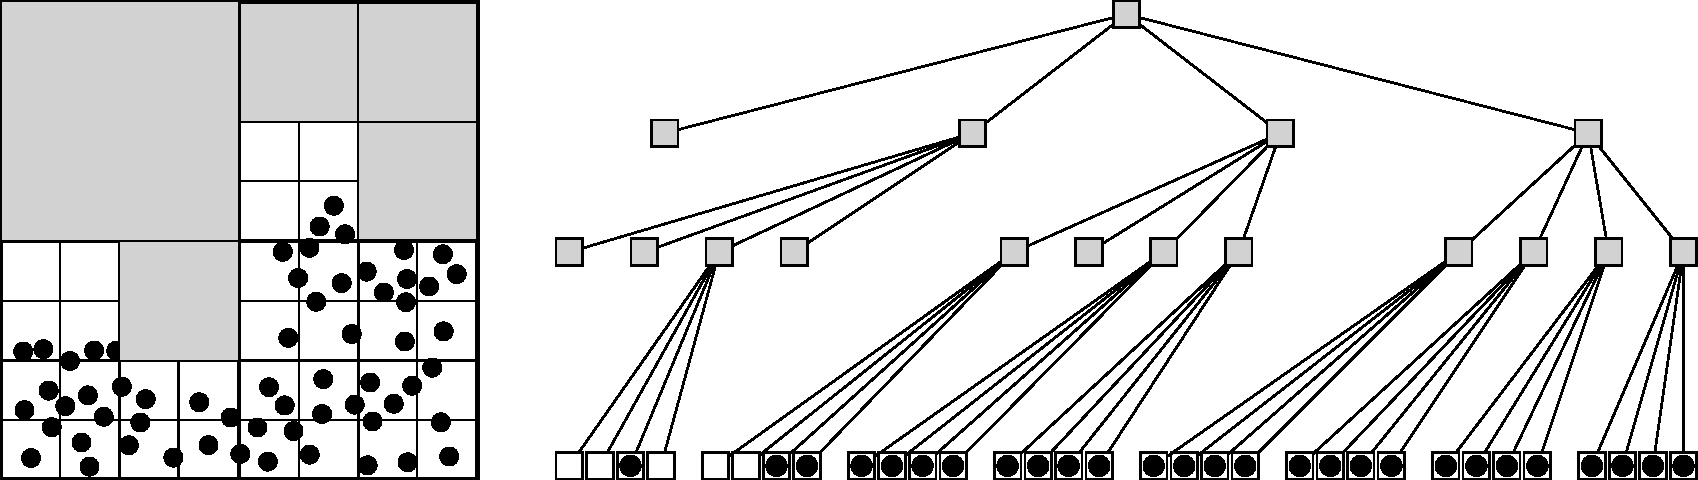
\includegraphics[width=\textwidth]{octree}
  \caption[Veranschaulichung der Funktionsweise eines Octrees]{
    Quadtree zur Veranschaulichung der Funktionsweise eines Octrees:\\
    Räumliche Unterteilung eines Raumes mit zugehörigem Baum von Zellen.
  }
  \label{fig:octree}
\end{figure}

%% \begin{algorithm}
%%   \begin{algorithmic}
%%     %    \Input $root$ - Stammzelle des Octrees
%%     %    \Input $i[3]$ - globale Adresse der Zielzelle
%%     %    \Input $allocate$ - Ob die Zelle neu erstellt werden soll
%%     \Result null falls leer, sonst Zielzelle
%%     \State
%%     \Function{getcell-octree}{$cell, id, allocate$}
%%     \State $d \gets $\Call{depth}{root}
%%     \Comment{Relative Tiefe, an der sich die Zielzellen befinden}
%%     \If{$d = 0$}
%%     \State\Return cell
%%     \EndIf
%%     \If{not $cell.children$}
%%     \If{allocate}
%%     \State $cell.children \gets $new cell[8]
%%     \Else
%%     \State \Return null
%%     \EndIf
%%     \EndIf
%%     \State $childid \gets $\Call{bitand}{id[0], $2^{d-1}$}
%%     + $2\cdot$\Call{bitand}{id[1], $2^{d-1}$}
%%     + $4\cdot$\Call{bitand}{id[2], $2^{d-1}$}
%%     %    \State \Comment{Indiziert die Subzelle aus der globalen Position}
%%     \State \Return\Call{getcell-octree}{$cell.children[childid], i, allocate$}
%%     \EndFunction
%%   \end{algorithmic}
%%   \caption[Zell-Adressierung in Octrees]{Rekursive Zell-Adressierung und -Allokierung im Octree: Bei jedem Schritt wird das Problem in 8 Unterzellen geteilt, woraus eine Laufzeit von \BigO{d}$=$\BigO{\log{c}} resultiert}
%%   \label{algo:octreeaddressing}
%% \end{algorithm}

\subsection{k-d-Bäume}
\label{datakdtree}

Für Nachbarschafts- und Bereichssuchen wird wegen ihrer hervorragenden Sucheffizienz oft auf k-d-Bäume zurückgegriffen, die einen kartesischen Raum in orthogonale Zellen mit jeweils einem Atom unterteilen, wodurch sich ein balancierter Binärbaum ergibt, an dessen Knoten die Atome liegen.
Durch implizite Betrachtung von Abstandsrelationen bei der Konstruktion (Abbildung~\ref{fig:kdtree}) lassen sich Abstands- oder Bereichssuchen in \BigO{\log{n}} durchführen, während Nachbarschaftssuchen von $N$ Atomen in Kombination mit einem Heap in \BigO{\log{n}\log{N}} möglich sind.

Nachteile ergeben sich bei Modifikationen von Atomen, die durch Baumrotation in \BigO{\log{n}} aufgelöst werden müssen und im schlimmsten Fall\footnote{Der schlimmste Fall (engl. \textit{worst case}) besteht in einer Menge von Eingabedaten, die zur größtmöglichen Laufzeit führen} den gesamten Baum neu strukturieren.
Durch die einseitige, dichte und gleichverteilte Hinzufügung von Atomen während einer Oberflächenabscheidung ist dieser Fall allerdings gegeben, da sich der Median der Atompositionen in z-Richtung stetig verschiebt.
Deshalb bieten sich k-d-Bäume zwar für allgemeine Suchoperationen in statischen Off-Lattice-Strukturen an, sind aber nicht für effiziente KMC-Simulationen geeignet.

\begin{figure}
  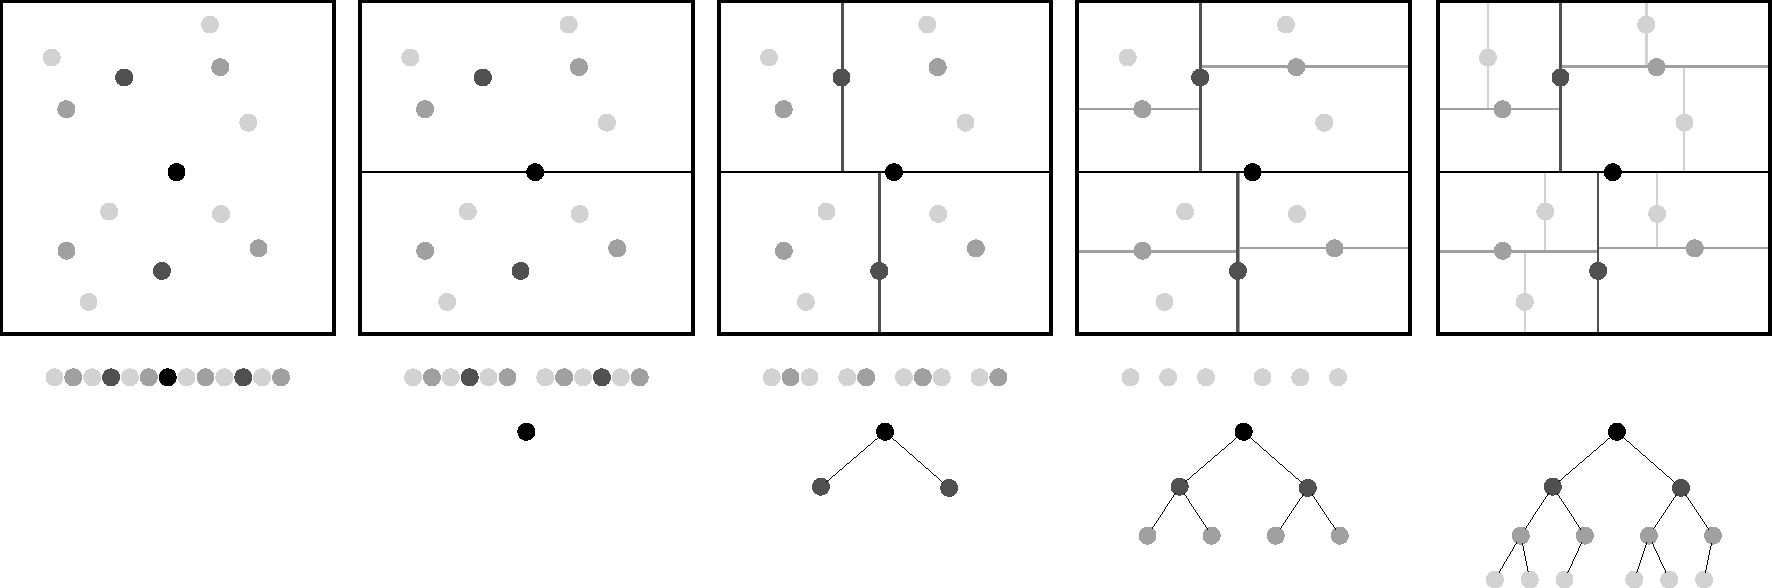
\includegraphics[width=\textwidth]{kdtree-tree}
  \caption[Konstruktion eines k-d-Baumes]{
    Konstruktion eines k-d-Baumes:
    Der Median der sortierten Punkte wird zur Wurzel des Baumes; die beiden Teilmengen rekursiv zu k-d-Bäumen
  }
  \label{fig:kdtree}
\end{figure}

%% \begin{algorithm}
%%   \begin{algorithmic}
%%     \Input $points$ - Liste von Punkten
%%     \Input $k$ - Dimensionalität des Simulationsraumes
%%     \Result Root-Element eines vollständigen k-d-Baumes aus diesen Punkten
%%     \State
%%     \Function{construct-kdtree}{$points, dim\gets0$}
%%     \State $n\gets$\Call{length}{points}
%%     \If{$n=0$}
%%     \State \Return null
%%     \Else
%%     \State \Call{sort}{$points, dim$} \Comment{Sortiert $points$ nach pos[$dim$]}
%%     \State $root\gets{}points\left[\lfloor\frac{n}{2}\rfloor\right]$
%%     \State $dim\gets(dim+1)\mod{k}$
%%     \State $root.left \gets$ \Call{construct-kdtree}{$points\left[0:\lfloor\frac{n}{2}\rfloor-1\right], dim$}
%%     \State $root.right \gets$ \Call{construct-kdtree}{$points\left[\lfloor\frac{n}{2}\rfloor+1:n-1\right], dim$}
%%     \State \Return $root$
%%     \EndIf
%%     \EndFunction
%%   \end{algorithmic}
%%   \caption[Konstruktion eines k-d-Baumes]{Rekursive Konstruktion eines k-d-Baumes (naive Implementierung)}
%%   \label{algo:kdtree-construction}
%% \end{algorithm}

\subsection{Delaunay-Triangulation}
\label{datadelaunay}

\begin{figure}
  \centering
  \def\svgwidth{\textwidth}
  \input{img/delaunay.pdf_tex}
  \caption[Beispiel des Delaunay-Kriteriums]{
    In der Delaunay-Triangulation (c) einer Punktwolke (a) dürfen sich keine weiteren Punkte im Umkreis jedes Simplexes (b) befinden
  }
  \label{fig:delaunay}
\end{figure}

Eine dritte Partitionsmethode findet sich in der Delaunay-Triangulation\todo{Ref?}, welche jedoch asymmetrisch und nicht-orthogonal arbeitet, indem die konvexe Hülle der Punktwolke raumfüllend in disjunkte k-dimensionale Simplexe\footnote{Ein $k$-Simplex ist ein Objekt in $k$ Dimensionen mit $k+1$ Eckpunkten, die untereinander mit geraden Kanten verbunden sind. Somit ist ein 1-Simplex eine Linie, ein 2-Simplex ein Dreieck, ein 3-Simplex ein Tetraeder, etc.}
entsprechend des Delaunay-Kriteriums, nach dem sich im Umkreis eines Simplexes keine anderen Punkte der Punktwolke befinden dürfen, zerlegt wird.
\todo{Anmerkung von Jörg: puuuhhh Du wirst hier ne ganze Menge Dine in den Raum, die eigentlich nach Erklärungen verlangen ...}
Damit ergibt sich ein Graph, der ein Supergraph des Nächstnachbargraphen\footnote{Der Nächstnachbargraph verbindet alle Punkte des Graphen mit ihrem nächsten Nachbarn}, der Alpha-Form (Abschnitt~\ref{dataalphaform}) sowie der konvexen Hülle\footnote{Die konvexe Hülle ist ein Körper aus Dreiecken, der alle Punkte der Punktwolke einschließt. Sie ergibt sich als Vereinigung einer vollständigen Triangulation. Siehe Abbildung~\ref{fig:delaunay-alpha-b}} der Punktwolke ist und in \BigO{n\log{n}} effizient konstruiert werden kann.
Die Konstruktion lässt sich im Gegensatz zu den anderen Datenstrukturen für große Simulationsräume mit entsprechenden Divide-and-Conquer-Algorithmen parallelisieren, oder vor einer etwaigen periodischen Erweiterung einer Einheitszelle zum Simulationsraum durchführen.
Eine Liste von Eigenschaften der Simplexe sowie einer Übersicht über die verschiedenen Konstruktionsmethoden ist in Anhang~\ref{appendix_delaunay} zu finden.

Delaunay-Triangulationen werden noch nicht direkt im KMC-Algorithmus für Off-Lattice-Systeme genutzt, doch sind sie aufgrund ihrer Beziehung zu Alpha-Formen für die Analyse von Oberflächen unentbehrlich (Abschnitt~\ref{mdmethods}).

\subsection{Alpha-Form}
\label{dataalphaform}

Delaunay-Triangulationen werden für Betrachtungen von Oberflächen interessant, da sie die konkave Oberfläche von Punktwolken über die Alpha-Form bestimmen können.
Sie werden durch Vereinigung genau der Simplexe konstruiert, deren Umkreisradius $r_d$ unterhalb einer frei wählbaren Grenze $\alpha$ liegt, oder durch komplementäre Algorithmen, wie sie in Abbildung~\ref{fig:delaunay-alpha} veranschaulicht sind.
Als Resultat ergibt sich eine Menge von Punkten und Dreiecken, welche die scheinbare Oberfläche der Punktwolke bilden, die für weitere Untersuchungen wie die Bestimmung von Oberflächenrauheiten genutzt werden kann.
Für Grenzwerte von $\alpha$ ergibt sich für $\alpha \rightarrow \infty$ die konvexe Hülle und für $\alpha \rightarrow 0$ die Gesamtheit der Atome.

Alpha-Formen beschreiben ebenfalls Hohlräume und Poren innerhalb der Struktur und können für $\alpha \approx r_\text{bond}$ sogar Kristalldefekte lokalisieren, die zuvor per Konnektivitätsprüfung der Alpha-Form \todo{Verweis auf Newman-Ziff-Algorithmus?} von der Oberfläche isoliert werden müssen.
Dabei sind Anwendungen auf auch periodische und teilperiodische Räume möglich.

%% Nachbarschaftssuche nicht notwendig

%% \subsubsection{Nachbarschaftssuche}
%% Für die Nachbarschaftssuche eines Referenzpunktes werden die raumfüllenden Eigenschaften der Triangulation relevant.
%% Der notwendigerweise konvexe, sonst aber beliebige Suchbereich um den Referenzpunkt wird von Simplexen überdeckt, die in direkter oder indirekter Nachbarschaft des Punktes liegen.
%% Somit teilen sich alle Punkte innerhalb des Suchbereiches eine Kante eines Simplexes mit einem anderen Punkt im Suchbereich, sofern der Suchbereich hinreichend groß ist.
%% Ausgehend vom Referenzpunkt sucht man entlang aller Kanten nach Punkten, die innerhalb des Suchbereiches liegen, bis alle potentiellen Punkte überprüft wurden.
%% Diese Vorgehensweise ist in Algorithmus~\ref{algo:delaunay-neigbors} ausführlich beschrieben.

%% \begin{algorithm}
%%   \centering
%%   \begin{algorithmic}
%%     \State Result = \{\}
%%     \State Queue = \{ P$_0$ : P$_0 \in$ Volume \}
%%     \While{Queue $\neq \emptyset$}
%%     \State Sei P $\in$ Queue
%%     \State Queue = Queue $\setminus$ \{ P \}
%%     \If{P $\in$ Volume}
%%     \State Result = Result $\cap$ \{ P \}
%%     \State Queue $\cap$ (Neighbors(P) $\setminus$ Result)
%%     \EndIf
%%     \EndWhile
%%   \end{algorithmic}
%%   \caption[Nachbarschaftssuche auf einer Delaunay-Triangulation]{Nachbarschaftssuche auf einer Delaunay-Triangulation.
%%     Ist der Suchraum konvex und hinreichend groß, lässt sich damit effizient nach Nachbarn eines bestimmten Punktes suchen.
%%   }
%%   \label{algo:delaunay-neighbors}
%% \end{algorithm}

\begin{figure}
  \centering
  \captionsetup[subfigure]{singlelinecheck=false}{
    \def\subwidth{0.4\textwidth}
    \def\svgwidth{\textwidth}
    \begin{subfigure}[t]{\subwidth}
      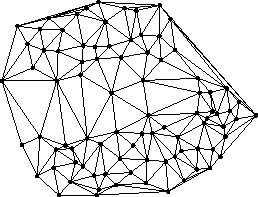
\includegraphics[width=\textwidth]{delaunay-alpha-a}
      \subcaption{Delaunay Triangulation einer beliebigen Punktmenge}
      \label{fig:delaunay-alpha-a}
    \end{subfigure}
    \hfill
    \begin{subfigure}[t]{\subwidth}
      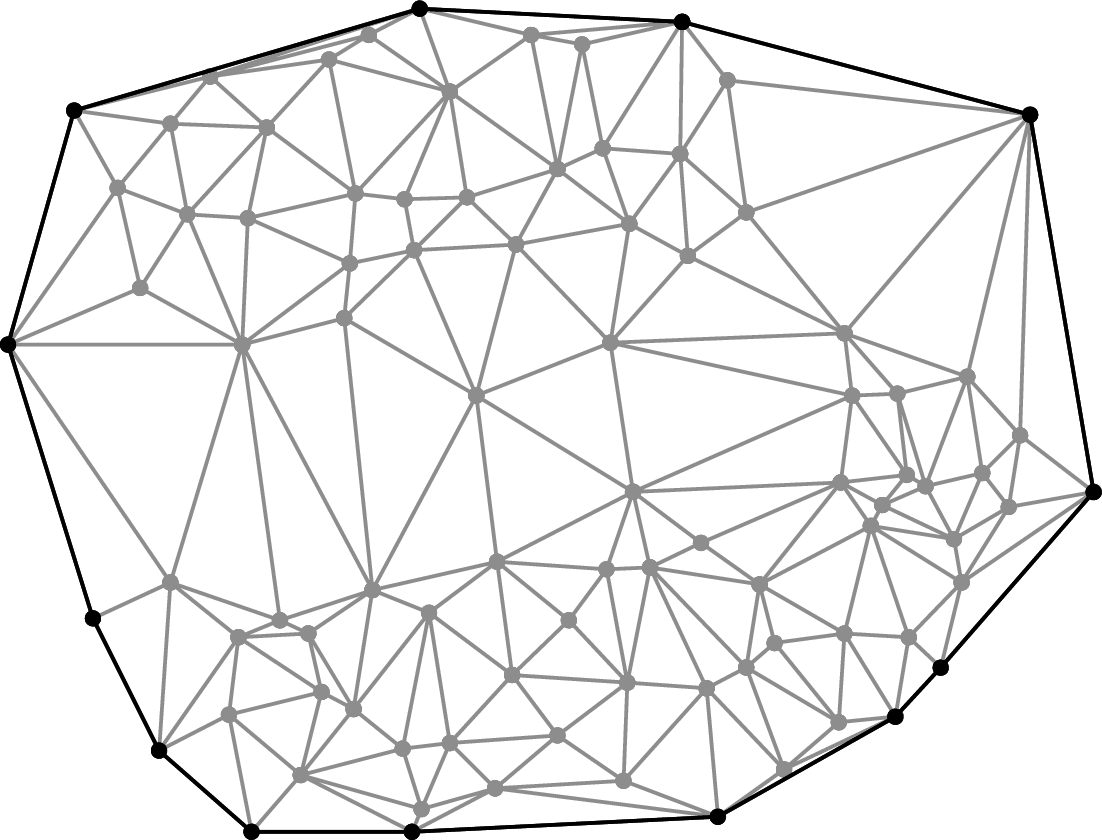
\includegraphics[width=\textwidth]{delaunay-alpha-b}
      \subcaption{Konvexe Hülle: Hülle der Triangulation}
      \label{fig:delaunay-alpha-b}
    \end{subfigure}
  }
  \vspace{2em}
  \captionsetup[subfigure]{singlelinecheck=false}{
    \def\subwidth{0.4\textwidth}
    \def\svgwidth{\textwidth}
    \begin{subfigure}[t]{\subwidth}
      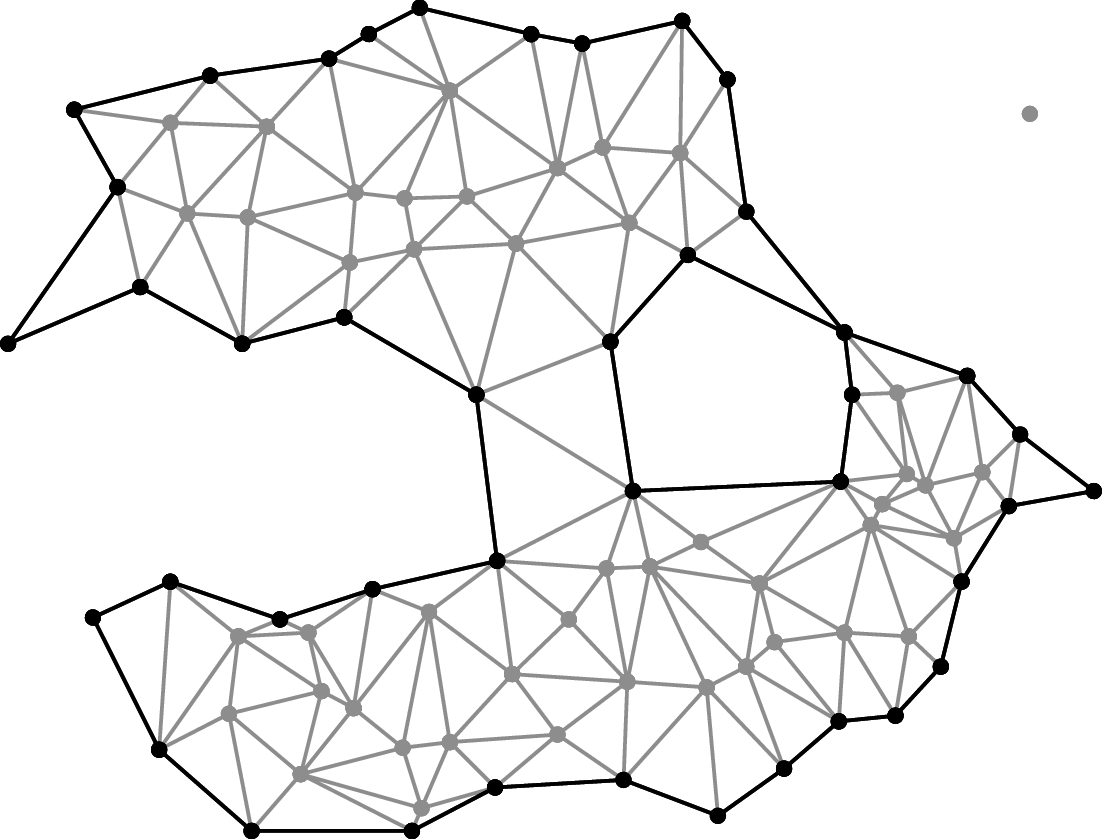
\includegraphics[width=\textwidth]{delaunay-alpha-c}
      \subcaption{Alpha-Form: Hülle nach Entfernung von Simplexen mit $r_d > \alpha$}
      \label{fig:delaunay-alpha-c}
    \end{subfigure}
    \hfill
    \begin{subfigure}[t]{\subwidth}
      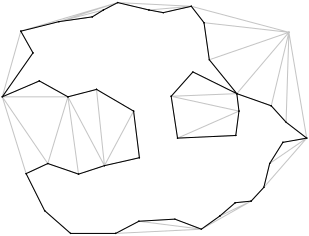
\includegraphics[width=\textwidth]{delaunay-alpha-d}
      \subcaption{Alpha-Form: Hülle nach Entfernung von Simplexen mit $r_d < \alpha$}
      \label{fig:delaunay-alpha-d}
    \end{subfigure}
  }
  \caption[Bestimmung der Oberfläche per Delaunay-Triangulation]{
    Bestimmung der Oberfläche per Delaunay-Triangulation.
    Die Alpha-Form in (d) trianguliert auch Ausreißer-Punkte, zählt sie aber ebenfalls nicht zur Hülle
  }
  \label{fig:delaunay-alpha}
\end{figure}

